\documentclass[12pt]{article}
\usepackage[left=1cm, right=1cm, top=2cm,bottom=1.5cm]{geometry} 

\usepackage[parfill]{parskip}
\usepackage[utf8]{inputenc}
\usepackage[T2A]{fontenc}
\usepackage[russian]{babel}
\usepackage{enumitem}
\usepackage[normalem]{ulem}
\usepackage{amsfonts, amsmath, amsthm, amssymb, mathtools}

\usepackage{fancyhdr}
\pagestyle{fancy}
\renewcommand{\headrulewidth}{1.5pt}
\renewcommand{\footrulewidth}{1pt}

\usepackage{graphicx}
\usepackage[figurename=Рис.]{caption}
\usepackage{subcaption}
\usepackage{float}

%%Наименование папки откуда забирать изображения
\graphicspath{ {./images/} }

%%Изменение формата для ввода доказательства
\renewcommand{\proofname}{$\square$  \nopunct}
\renewcommand\qedsymbol{$\blacksquare$}

\addto\captionsrussian{%
	\renewcommand{\proofname}{$\square$ \nopunct}%
}
%% Римские цифры
\newcommand{\RN}[1]{%
	\textup{\uppercase\expandafter{\romannumeral#1}}%
}


\theoremstyle{definition}
\newtheorem{defn}{Опр:}
\newtheorem{rem}{Rm:}
\newtheorem{prop}{Утв.}
\newtheorem{exrc}{Упр.}
\newtheorem{lemma}{Лемма}
\newtheorem{theorem}{Теорема}
\newtheorem{corollary}{Следствие}

\newenvironment{cusdefn}[1]
{\renewcommand\thedefn{#1}\defn}
{\enddefn}



\DeclareRobustCommand{\divby}{%
	\mathrel{\text{\vbox{\baselineskip.65ex\lineskiplimit0pt\hbox{.}\hbox{.}\hbox{.}}}}%
}


\newcommand{\smallerrel}[1]{\mathrel{\mathpalette\smallerrelaux{#1}}}
\newcommand{\smallerrelaux}[2]{\raisebox{.1ex}{\scalebox{.75}{$#1#2$}}}

\newcommand{\smallin}{\smallerrel{\in}}
\newcommand{\smallnotin}{\smallerrel{\notin}}

\begin{document}
	\lhead{Математический анализ - I}
	\chead{Шапошников С.В.}
	\rhead{Лекция - 11}

\begin{theorem}\textbf{(Критерий Коши для рядов)}:\\
	$\displaystyle \sum\limits_{n=1}^{\infty} a_n$ - сходится $\Leftrightarrow \forall \varepsilon >0, \exists \, N \colon \forall n,m > N, \, |S_n - S_m| = \Bigg|\displaystyle \sum\limits_{k = m+1}^{n}{a_k}\Bigg|  < \varepsilon$.
\end{theorem}

Без доказательства, так как сходимость $S_n$ - есть сходимость ряда.

\begin{corollary}
	Если ряд $\displaystyle \sum\limits_{n=1}^{\infty} |a_n|$ сходится, то  $\displaystyle \sum\limits_{n=1}^{\infty} a_n$ сходится.
\end{corollary}

\begin{proof}
	Для $\displaystyle \sum\limits_{n=1}^{\infty} |a_n|$ выполняется условие Коши $\Rightarrow \forall \varepsilon > 0, \exists \, N \colon \forall n, m > N, \,
	\Bigg|\displaystyle \sum\limits_{k = m+1}^{n} |a_k| \Bigg| < \varepsilon \Rightarrow$ по неравенству треугольника $\Bigg|\displaystyle \sum\limits_{k = m+1}^{n} a_k \Bigg| \leq \displaystyle \sum\limits_{k = m+1}^{n} |a_k| = \Bigg|\displaystyle \sum\limits_{k = m+1}^{n} |a_k| \Bigg| < \varepsilon \Rightarrow$ для $\displaystyle \sum\limits_{k = 1}^{\infty} a_k$ выполняется условие Коши.
\end{proof}

\begin{rem}
	Обратное утверждение - не верно.
\end{rem}

\textbf{Пример}: (Ряд Лейбница) $\displaystyle \sum\limits_{n=1}^{\infty} \frac{(-1)^n}{n}$ - знакопеременный ряд. Он сходится, проверим сходимость с помощью критерия Коши, пусть $m\leq n$: $$\bigg| \dfrac{(-1)^{m+1}}{m+1} + \dfrac{(-1)^{m+2}}{m+2} + \dotsc + \dfrac{(-1)^n}{n} \bigg| \leq \bigg|\dfrac{(-1)^{m+1}}{m+1} + \dfrac{(-1)^{m+2}}{m+2} \bigg| + \bigg|\dfrac{(-1)^{m+3}}{m+3} + \dfrac{(-1)^{m+4}}{m+4} \bigg| + \dotsc + \bigg(\dfrac{1}{n} \bigg)=$$ 
$$= \dfrac{1}{m+1} - \dfrac{1}{m+2} + \dfrac{1}{m+3} - \dfrac{1}{m+4} + \dotsc \bigg(\pm \dfrac{1}{n} \bigg) \leq \dfrac{1}{m+1}$$ 

Если нечетное число слагаемых, то $\frac{1}{n}$ идет со знаком $+$, если четное число слагаемых, то со знаком $-$.
Группируем следующие слагаемые:
$$\dfrac{1}{m+1} \underbrace{ - \dfrac{1}{m+2} + \dfrac{1}{m+3}}_{\leq 0} \underbrace{- \dfrac{1}{m+4} + \dfrac{1}{m+5}}_{\leq 0}+ \dotsc \bigg(\pm \dfrac{1}{n} \bigg) \leq \dfrac{1}{m+1}$$

Если количество нечетное, то все разобьется по парам. Если количество четное, то будет $-\frac{1}{n} <0$ и можно слагаемое не рассматривать.

$$\forall \varepsilon > 0, \exists \, N, (N > \frac{1}{\varepsilon}), \forall n,m > N, \, \bigg|\dfrac{(-1)^{m+1}}{m+1} + \dotsc + \dfrac{(-1)^n}{n} \bigg| < \varepsilon$$.
 
\begin{rem}
	$x_n = (x_n - x_{n-1}) + (x_{n-1} - x_{n-2}) + \dotsc + (x_2 - x_1) + x_1 = a_n + a_{n-1} \dotsc + a_2 + a_1$, тогда $\lim\limits_{n \to \infty} x_n = \sum\limits_{n=1}^{\infty} a_n$.
\end{rem}

Таким образом, все что умеем для рядов - умеем делать и для последовательностей и наоборот.

\textbf{Пример}: $|x_n - x_{n-1}| \leq \frac{1}{2^n} \Rightarrow \exists\, \lim\limits_{n\to \infty} x_n$. Тогда, если $x_n =a_n + a_{n-1} \dotsc + a_2 + a_1$, то $|a_n| \leq \dfrac{1}{2^n} \Rightarrow$ \\
$\Rightarrow \displaystyle \sum\limits_{n=1}^{\infty} |a_n|$ - сходится $\Rightarrow \displaystyle \sum\limits_{n=1}^{\infty} a_n$ - сходится $\Rightarrow \exists\, \lim\limits_{n\to \infty} x_n$.

\newpage

\section*{Топология вещественной прямой $\mathbb{R}$}

\begin{defn}
	\uwave{Окрестность точки} $a$ - это произвольный интервал, содержащий $a$, пишут $\mathcal{U}(a)$.
\end{defn}

\begin{figure}[H]
	\centering
	\includegraphics[width=0.2\textwidth]{11_1.eps}
	\caption{Окрестность точки $a$.}
	\label{11_1}
\end{figure}

\begin{defn}
	\uwave{Проколотая окрестность} $\mathcal{U}^\prime(a) = \mathcal{U}(a) \setminus \{a\}$.
\end{defn}

\begin{figure}[H]
	\centering
	\includegraphics[width=0.2\textwidth]{11_2.eps}
	\caption{Проколотая окрестность точки $a$.}
	\label{11_2}
\end{figure}

Будем использовать обозначение $\mathcal{U}_\varepsilon(a) = (a- \varepsilon, a+ \varepsilon)$ и $\mathcal{U}_\varepsilon^\prime(a) = \mathcal{U}_\varepsilon(a) \setminus \{a\}$.

В любом интервале, можно найти симметричный интервал.
\begin{figure}[H]
	\centering
	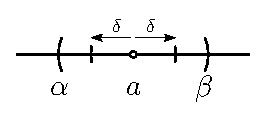
\includegraphics[width=0.2\textwidth]{11_3.eps}
	\caption{Симметричная окрестность точки $a$.}
	\label{11_3}
\end{figure}


\begin{defn}
	Множество $V \subset \mathbb{R}$ называется \uwave{открытым}, если $\forall a \in V, \exists \, \mathcal{U}(a) \subset V$.
\end{defn}

\textbf{Примеры}: интервал, \uline{вещественная прямая}, \uline{пустое множество} - открытые множества.

\begin{figure}[H]
	\centering
	\includegraphics[width=0.5\textwidth]{11_4.eps}
	\caption{Примеры открытых множеств: интервал, вещественная прямая, пустое множество.}
	\label{11_4}
\end{figure}

\begin{defn}
	Множество $F\subset \mathbb{R}$ называется \uwave{замкнутым}, если $\mathbb{R} \setminus F$ - открытое.
\end{defn}

\textbf{Примеры}: точка, \uline{вещественная прямая}, \uline{пустое множество}, отрезок - замкнутые множества.

\begin{figure}[H]
	\centering
	\includegraphics[width=0.7\textwidth]{11_5.eps}
	\caption{Примеры замкнутых множеств: точка, отрезок, вещественная прямая, пустое множество.}
	\label{11_5}
\end{figure}

$\mathbb{R}$ - замкнутое, потому что оно дополнение к пустому множеству. \\
$\varnothing$ - замкнутое, так как оно дополняет числовую прямую.

Пример ни замкнутого, ни открытого множества - полуинтервал.

\begin{figure}[H]
	\centering
	\includegraphics[width=0.2\textwidth]{11_6.eps}
	\caption{Полуинтервал}
	\label{11_6}
\end{figure}


\begin{theorem}\hfill
	\begin{enumerate}[label={\arabic*)}]
		\item Объединение \uline{всякого набора} открытых множеств и \uline{пересечение конечного набора} открытых множеств является \uwave{открытым} множеством.
		\item Объединение \uline{конечного набора} замкнутых множеств и пересечениие \uline{всякого набора} замкнутых множеств является \uwave{замкнутым} множеством.
	\end{enumerate}
\end{theorem}

\begin{proof}\hfill
	\begin{enumerate}[label={\arabic*)}]
		\item Пусть $\{V_\alpha\}_{\alpha \smallin A}$ - открытые множества. Пусть $a \in \bigcup\limits_\alpha V_\alpha \Rightarrow \exists \, \alpha \colon a \in V_\alpha$, но по условию $V_\alpha$ - открытое множество $\Rightarrow \exists \, \mathcal{U}(a) \colon \mathcal{U}(a) \subset V_\alpha \Rightarrow \mathcal{U}(a) \subset \bigcup\limits_\alpha V_\alpha \Rightarrow \bigcup\limits_\alpha V_\alpha$ - открытое множество по определению.\\
		$V_1,\dotsc, V_N$ - открытые множества. Пусть $a \in \bigcap\limits_{n=1}^{N} V_n \Rightarrow a \in V_n, \, \forall n = 1, \dotsc, N \Rightarrow$\\ $\Rightarrow \exists \, \mathcal{U}_{\varepsilon_1}(a) \subset V_1, \exists \, \mathcal{U}_{\varepsilon_2}(a) \subset V_2, \dotsc, \exists \, \mathcal{U}_{\varepsilon_N}(a) \subset V_N$. Пусть $\varepsilon = \min\{\varepsilon_1, \varepsilon_2, \dotsc, \varepsilon_N \} \Rightarrow \mathcal{U}_\varepsilon(a) \subset \mathcal{U}_{\varepsilon_n}(a), \, \forall n = 1, \dotsc, N$. Тогда $\mathcal{U}_\varepsilon(a) \subset V_n, \, \forall n = 1, \dotsc, N \Rightarrow \mathcal{U}_\varepsilon(a) \subset \bigcap\limits_{n=1}^{N} V_n$. Пересечение конечного набора необходимо, чтобы можно было найти минимум из $\varepsilon_n$.
		
		\item Выводится из $1)$ формулами Моргана: $\mathbb{R} \setminus(\bigcap\limits_\alpha F_\alpha) = \bigcup\limits_\alpha(\underbrace{\mathbb{R} \setminus F_\alpha}_{\text{откр.}})$ - открытое, как объединение открытых множеств $\Rightarrow \bigcap\limits_\alpha F_\alpha$ - замкнутое множество.\\		
		Выводится из $1)$ формулами Моргана: $\mathbb{R} \setminus (\bigcup\limits_{n=1}^{N} F_n) = \bigcap\limits_\alpha(\underbrace{\mathbb{R} \setminus F_\alpha}_{\text{откр.}})$ - открытое, как конечное пересечение открытых множеств $\Rightarrow \bigcup\limits_{n=1}^{N} F_n$ - замкнутое множество.
	\end{enumerate}
\end{proof}

\begin{defn}
	Если в некотором непустом множестве $X$ выделен набор подмножеств $\tau$:
	\begin{enumerate}[label={(\arabic*)}]
		\item $X, \varnothing \in \tau$;\\
		\item $V_\alpha \in \tau \Rightarrow \bigcup\limits_{\alpha} V_\alpha \in \tau$;
		\item $V_1, \dotsc, V_n \in \tau, \, \bigcap\limits_{n=1}^{N} \in \tau$;
	\end{enumerate}
	то говорят, что на $X$ задана топология $\tau$. А элементы этого набора называют \uwave{открытыми множествами}.
\end{defn}

\begin{theorem}
	Непустое открытое множество в $\mathbb{R}$ является объединением не более, чем счетного набора попарно непересекающихся интервалов (возможно с бесконечными концами). 
\end{theorem}

\begin{proof}
	Пусть $V$ - открыто, $V \neq \varnothing$. Пусть $a \in V$, рассмотрим множество $E^{+} = \{\, x > a \colon (a,x) \subset V \,\}$. $E^{+}  \neq \varnothing$, так как $\exists \, (\alpha, \beta) \subset V \colon a \in (\alpha, \beta), \, \beta \in E^{+}$. Тогда
	\begin{enumerate}[label={\arabic*)}]
		\item $E^+$ не ограничено сверху $\Rightarrow$ пусть $x_0 > a$, так как $E^+$ - не ограничено сверху, то $\exists \, x \in E^+ \colon x > x_0 \Rightarrow (a,x) \subset V \Rightarrow x_0 \in V$. Таким образом, любая точка справа от $a$ лежит в $V \Rightarrow (a, +\infty) \subset V$.
		
		\item $E^+$ ограничено сверху $\Rightarrow$ по принципу полноты Вейрштрасса $B = \sup{E^+} \Rightarrow (a, B) \subset V$ и $B \notin V$. $\forall \varepsilon > 0, \, B - \varepsilon$ - не является верхней гранью $E^+$, то есть $\exists \, x \in E^+ \colon x > B - \varepsilon \Rightarrow B - \varepsilon \in (a,x) \subset V$, если $B - \varepsilon > a$. Все такие $B - \varepsilon > a$ элементы находятся в интервале $(a, B)$. Если $B \in V$, то $\exists \, \varepsilon > 0 \colon (B - \varepsilon, B + \varepsilon) \subset V \Rightarrow (a, B + \varepsilon) \subset V \Rightarrow B + \varepsilon \in E^+$ - а это противоречит тому, что $B = \sup{E^+}$.
	\end{enumerate} 

	Получили $(a, B) \subset V, \, B = +\infty$ или $B \notin V$. Аналогично строим $(C,a) \subset V, \, C = -\infty$ или $C \notin V$. 
	
	Таким образом, для всякой точки $a \in V$ построен интервал $a \in (C,B) \subset V$ и $C, B \notin V$ или $\pm \infty$.
	
	Пусть $(C_1, B_1)$ и $(C_2, B_2)$ - два таких интервала. Предположим, что они не совпадают, но пересекаются: конец одного из них принедлежит другому. Пусть $C_1 \in (C_2, B_2)$, тогда (остальные случаи - аналогично) $C_1 \in V$, но по построению $C_1 \notin V \Rightarrow$ противоречие $\Rightarrow$ интервалы либо не пересекаются, либо совпадают.
	
	Покажем, что на $\mathbb{R}$ можно расположить не более чем счетный набор попарно не пересекающихся интвервалов. Пусть есть такой набор интервалов $\{I_\alpha\} \colon I_\alpha \cap I_\beta = \varnothing$, где $\alpha \neq \beta$. $$\forall \alpha, \exists \, r_\alpha \in \mathbb{Q} \colon r_\alpha \in I_\alpha$$
	
	\uwave{Идея}: есть интервал (пусть лежит справа от нуля) длины $l$. По аксиоме Архимеда возьмем такое $n \colon \frac{1}{n} < l$ и начнем идти от $0$ в сторону интервала с шагом $\frac{1}{n}$. По аксиоме Архимеда мы должны перепрыгнуть левую точку интервала: обязательно найдется такое $m$, что $\frac{m}{n} >$ левая точка интервала, но при этом $\frac{m}{n} <$ правой точки интервала, так как шаг с которым идем короче этого интервала. Получим $r$ - искомое рациональное число. В каждом интервале есть рациональная точка. 
	
	\begin{figure}[H]
		\centering
		\includegraphics[width=0.34\textwidth]{11_7.eps}
		\caption{Существование рационального числа.}
		\label{11_7}
	\end{figure}
	
	Заметим, что если $\alpha \neq \beta \Rightarrow r_\alpha \neq r_\beta$, т.к. $I_\alpha \cap I_\beta = \varnothing$. Таким образом, есть отображение $I_\alpha \mapsto r_\alpha \in \mathbb{Q}$ - инъекция $\Rightarrow$ т.к. это инъекция в счетное множество, то $\{I_\alpha\}$ - не более, чем счетен.
\end{proof}

\end{document}